\documentclass{article}
\usepackage[sglblindworkshop,final]{neurips_2026}
\workshoptitle{Interpreting Agent Behavior}

\usepackage[utf8]{inputenc}
\usepackage[T1]{fontenc}
\usepackage[hidelinks]{hyperref}
\usepackage{url,booktabs,amsfonts,amsmath,amssymb,nicefrac,microtype,xcolor,graphicx,float,tabularx,array,enumitem}
\usepackage{rotating}
\usepackage{tikz}
\renewcommand{\ttdefault}{lmtt}
\usetikzlibrary{arrows.meta,positioning,fit,calc}
\graphicspath{{figs/}}

\renewcommand{\topfraction}{0.95}\renewcommand{\bottomfraction}{0.7}\renewcommand{\textfraction}{0.05}\renewcommand{\floatpagefraction}{0.8}
\setcounter{topnumber}{3}\setcounter{bottomnumber}{2}\setcounter{totalnumber}{4}
\setlength{\textfloatsep}{10pt plus 2pt minus 2pt}\setlength{\floatsep}{8pt plus 2pt minus 2pt}\setlength{\intextsep}{8pt plus 2pt minus 2pt}
\setlength{\abovecaptionskip}{4pt}\setlength{\belowcaptionskip}{0pt}
\newcolumntype{Y}{>{\raggedright\arraybackslash}X}
\newcommand{\q}{^{*}}          % BH-FDR q < 0.05
\newcommand{\ua}{^{\dagger}}   % unadjusted CI excludes zero

\title{Steered affect moves a partner agent's activations, and the logistic probe that reads it returns a tie-break, not an estimate}

\author{%
  Manan Wadhwa\thanks{Co-first authors.}\hspace{0.55em} Shivam Dubey\footnotemark[1]\hspace{0.55em} Debojeet Ghosh\hspace{0.55em} Shreyansh Kumar\hspace{0.55em} Ayushman Garg \\
  Redarc Labs \\
  \texttt{manan@redarclabs.com} \quad \texttt{shivam@redarclabs.com}
}

\begin{document}
\maketitle

% ---------------------------------------------------------------------------------------
% Abstract, Introduction and Setup: authors' text (typo-level corrections only).
% ---------------------------------------------------------------------------------------
\begin{abstract}
We steered an LLM agent towards an emotion and a second agent talked to it. A linear probe inside that second agent, for that emotion, read higher when the first agent was steered more strongly, and this held for five of six emotions on Qwen3.6-27B and Llama-3-8B-Instruct-abliterated. We also found that standard methods are misleading: the usual way of finding an emotion's direction returns unstable directions, and the usual control is too weak. When fitted on two separate halves of our data, logistic regression returns directions that do not agree with each other, but directions built from the difference between the emotions' average activations agree very closely (cosine similarity of 0.57 and 0.29 vs.\ 0.97 and 0.94 for the 27B and 8B models, respectively). When there are fewer examples than activation dimensions, logistic regression separates the training data perfectly, so its direction is not set by the data itself but by its penalty. We also tested whether the stable direction carries the emotion. To do this, we erased it where the second agent reads the first agent's message and then measured whether the reading stops rising. Across emotions, a median 91\% of the effect remains. Erasing a random region, which is what is usually done, does nothing, but a region built using shuffled emotion labels reduced the effect for three emotions, whereas the real region that holds the six emotion directions reduced it for only two. This would have been missed by a random control. A probe cannot tell whether it is reading the second agent's emotions or just a picture of the first agent's.
\end{abstract}

\section{Introduction}
Systems of several language-model agents are common \citep{guo2024multiagent}, and affect has begun to be studied as it moves between such agents, by expression in crowd simulations \citep{durupinar2026affect} and by emotion policies in negotiation \citep{long2025evoemo}. If one agent is in an emotional state, does anything of that state reach another's internal representation? A transfer that changes the receiver's internal representation need not show in transcripts, which we do not examine here, and is visible in activations, which makes it a question for representation-level tools: steering vectors to induce a state in the sender \citep{turner2023actadd,rimsky2023caa,zou2023repe,li2023iti,sofroniew2026emotion,jeong2026emotion}, probes to read it in the receiver, and ablations to test what carries it.

Those tools rest on one object, a direction in activation space, which has to be trusted twice: once to read and once to intervene. Our claim is that both uses fail in ways the usual checks miss. Read with a logistic-regression coefficient row, the direction does not reproduce across independent fits. The reason is separability, which no sample size within reach ($n \le 2000$ against $d = 5120$) and no penalty schedule removes: the fitted row is a tie-break among separating hyperplanes, not an estimate \citep{rosset2004margin,soudry2018implicit,marks2023geometry}. Intervene with the reproducible direction, and the standard control, a norm-matched random vector, stays inert, while a rank-5 subspace fitted by the same estimator on destroyed labels blocks the response at the same false-discovery threshold as the affect subspace does.

The evidence is an estimator study across two models and three depths, and three pre-registered experiments on the channel, each critiqued blind before its wording entered this paper. The response itself survives resampling: five of six emotions respond on each model. The channel is not what the linear picture suggests. Removing the emotion direction everywhere it can be read leaves most of the response; only sad loses at least 24\% against the permuted-label control (23\% against baseline) in every one of ten direction draws, and afraid 18\% at the median with its manipulation check passing in four draws of ten. A rank-5 affect subspace cannot serve as an instrument because it shifts the readout used to check it. A rank-1 permuted-label direction is inert while a rank-5 permuted-label frame is not.

The practical consequence is a change to the controls register of any ablation study of a concept direction: beside the random direction, run the same estimator on permuted labels at the rank of the intervention, report every arm's footprint, and check the manipulation with an instrument that does not share the ablation's target. The scientific consequence is narrower than we hoped: the receiver's response exists, the rank-1 direction carries part of it for sad on both models and across direction draws, less reliably for afraid, and the rest is open.

\paragraph{Contributions.}
\begin{itemize}[leftmargin=1.2em,itemsep=1pt,topsep=2pt]
\item Dose-responsive movement of the receiver's present-emotion projection for five of six emotions on two models, with common-random-number sampling and scenario-blocked inference; the other-speaker projection moves comparably, which bounds the construct claim (Section~\ref{sec:transfer}).
\item Disjoint-half reproducibility of probe directions as the missing quantity: logistic 0.57 / 0.29 against difference-of-means 0.97 / 0.94, unchanged by a fixed per-sample penalty, with the mechanism (perfect separation at every $n$; the direction is the penalty's tie-break and drifts from the mean difference) measured directly, and its downstream cost bounded by held-out accuracy and projection correlation (Section~\ref{sec:estimator}).
\item Three pre-registered ablations with their verdicts as registered: rank-1 insufficiency (H1), rank-5 instrument failure, and survival of the rank-1 block against a permuted-label rank-1 control (H3), with two of the designs rerun on the second model, where only sad's result carries over (Section~\ref{sec:ablations}).
\item Every arm against baseline in one table with one significance standard, including the two random controls the argument depends on, and the resulting rule for controls (Section~\ref{sec:controls}).
\end{itemize}
Every number is registered with a pointer to the committed script and result file that produced it (Appendix~\ref{app:registry} maps each number to its identifier). Seven of our own interpretive sentences were withdrawn under blind critique and the reviews of the first version forced eighteen more corrections; both lists are in the supplementary material.

\paragraph{Relation to prior work.} That logistic probe directions can be unstable is not our discovery, nor is rank-1 insufficiency under ablation \citep{elazar2021amnesic,ravfogel2020inlp,belrose2023leace}; the permuted-label control is the intervention analogue of the control task \citep{hewitt2019control}. \citet{marks2023geometry} identified the deficiency and proposed mass-mean probing, noting that logistic regression converges toward the maximum-margin separator on separable data, the implicit bias analysed by \citet{soudry2018implicit}; \citet{gao2026raptor} name directional stability as a requirement for probe-then-steer pipelines and propose ridge-tuned logistic regression, reporting mean pairwise robustness of 0.87--0.98 under 20\% training-data ablations. Our contribution is the quantity: reproducibility across \emph{disjoint} halves, which share no examples where two 80\% subsamples share most, plateaus at 0.55--0.61 on the 27B and falls to 0.28--0.38 on the 8B while difference-of-means rises to 0.94--0.98 on the same splits. \citet{braun2025unreliability} corroborate for mean-difference steering vectors, which vary widely from 5--30 training samples and agree above 0.99 from 200--500, the estimator we also find reproducible. \citet{herbster2026steering} report mean-difference and logistic directions near-identical for compassion (0.98--0.99, on the same Qwen3.6-27B) but 0.80 for one honesty case; at their training-set sizes our cosine is also above 0.9 (Figure~\ref{fig:estimator}c), and at $n=2000$ we find 0.43 and 0.33--0.37, so the results are consistent with drift in $n$. \citet{raju2026geometric} measure stability across feature dimensions, a different axis.

\section{Setup}
\label{sec:setup}
\begin{figure}[t]
\centering
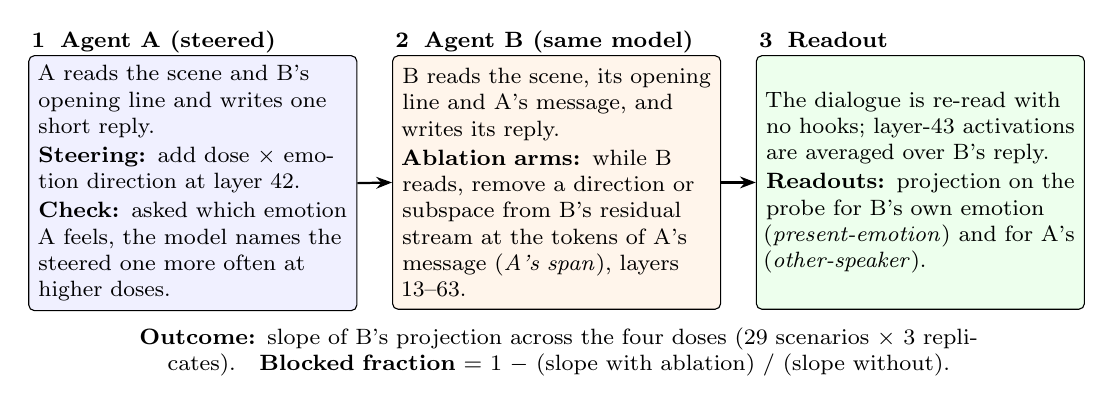
\begin{tikzpicture}[
  font=\footnotesize,
  box/.style={draw, rounded corners=2pt, align=left, inner sep=3.5pt, text width=3.92cm, minimum height=3.22cm, anchor=north west, fill=#1},
  lab/.style={font=\footnotesize\bfseries, anchor=south west, inner sep=1pt, text depth=0.4ex},
  arr/.style={-{Stealth[length=2mm]}, line width=0.8pt}]
\node[box=blue!6] (A) at (0,0) {A reads the scene and B's opening line and writes one short reply.\\[1pt]
\textbf{Steering:} add dose $\times$ emotion direction at layer 42.\\[1pt]
\textbf{Check:} asked which emotion A feels, the model names the steered one more often at higher doses.};
\node[box=orange!8] (B) at (4.62,0) {B reads the scene, its opening line and A's message, and writes its reply.\\[1pt]
\textbf{Ablation arms:} while B reads, remove a direction or subspace from B's residual stream at the tokens of A's message (\emph{A's span}), layers 13--63.};
\node[box=green!7] (R) at (9.24,0) {The dialogue is re-read with no hooks; layer-43 activations are averaged over B's reply.\\[1pt]
\textbf{Readouts:} projection on the probe for B's own emotion (\emph{present-emotion}) and for A's (\emph{other-speaker}).};
\node[lab] at (A.north west) {1\;\;Agent A (steered)};
\node[lab] at (B.north west) {2\;\;Agent B (same model)};
\node[lab] at (R.north west) {3\;\;Readout};
\draw[arr] (A.east) -- (B.west);
\draw[arr] (B.east) -- (R.west);
\node[anchor=north, text width=13.2cm, align=center] at ($(B.south)+(0,-0.1)$) {\textbf{Outcome:} slope of B's projection across the four doses (29 scenarios $\times$ 3 replicates).\quad \textbf{Blocked fraction} = 1 $-$ (slope with ablation) / (slope without).};
\end{tikzpicture}
\caption{\textbf{Setup.} One model plays both agents and neither has a system persona: each turn is a plain-text prompt that gives one of 29 everyday scenes (for example, two coworkers talking after a long shift), B's opening line, and an instruction to write the next speaker's reply as one short paragraph; the two names rotate across replicates. A's message is the same in every ablation arm, so differences between arms come from what B does with it.}
\label{fig:setup}
\end{figure}

Two agents, A and B, converse in 29 fixed scenarios. A's message is generated under a steering vector added at layer 42 of Qwen3.6-27B (revision \texttt{6a9e13bd}) at a steering strength (which we call the ``dose'') of 0, 0.33, 0.67 or 1.0 times a fixed scale (the activation RMS at the focus layer), with three replicate seeds; B's reply is then sampled with common random numbers across experimental arms, so that sampling noise shared between two arms cancels inside each paired contrast. There are two readouts in the paper. One is B's \emph{present-emotion projection}, which is the projection of B's reply activations on a difference-of-means probe for B's own emotion. The other is B's \emph{other-speaker projection}, on the matching probe for the interlocutor's emotion. Both probes are fitted on one half (808 items) of a 1,615-item probe pool, while the steering and ablation directions are fitted, per layer, on the disjoint other half (807 items). A generation-side forced-choice readout of A's span is the manipulation check. Every dose-response slope is an ordinary least-squares slope over the four doses on per-scenario means, which means two things: every confidence interval is a scenario-blocked percentile bootstrap \citep{efron1993bootstrap} (29 clusters, 5,000 draws), and every between-arm contrast is scenario-blocked and dose-paired. We use Benjamini--Hochberg \citep{benjamini1995fdr} false-discovery rates within one family of five testable emotions unless stated otherwise.

\paragraph{Two pools.} The estimator study (Section~\ref{sec:estimator}) uses a separate, larger generation pool built for it with the same generator as the probe pool (six present emotions $\times$ six interlocutor emotions, 160 dialogues per cell on the 27B (220 on the 8B) instead of 60, degenerate and refusing outputs dropped): 4,253 items on the 27B (kept from 5,760 generated) and 3,898 on the 8B, with no items in common with the 1,615-item probe pool, so that disjoint halves of up to 2,000 items exist on the 27B; on the 8B two halves of 1,949 would fit but the next point of the pre-declared grid (2,000) does not, so its curves stop at 1,200. The second model is Llama-3-8B-Instruct-abliterated (revision \texttt{dd67dd05}); its runs are out-of-pre-registration replications with a weaker, less specific manipulation (Section~\ref{sec:ablations}). The ablation experiments use the 1,615-item probe pool above, on which the deployed directions' own split-half cosine at 600 per half is 0.88--0.93 across the ablated layers (the pre-registered gate).

\paragraph{Footprint.} For every ablation arm we record the norm of the component removed from A's residual stream, averaged over the masked positions and the ablated layers; all ratios are relative to the emotion direction's value in the same run (Table~\ref{tab:dirs}). It measures how much an arm perturbs the residual stream, so a control that blocks only because it removes more can be told apart: B1c's random direction removes 2.0$\times$ the emotion direction's footprint and blocks nothing, while the permuted-label frame removes 11$\times$.

% ---------------------------------------------------------------------------------------
\section{Which direction can be trusted?}
\label{sec:estimator}
Everything that follows needs one direction per emotion: to steer A, to read B and to erase. This section asks which way of finding that direction gives the same answer twice. We compare two estimators, both fitted on standardised activations (each coordinate divided by its standard deviation). \emph{Logistic regression}, the usual choice in probe studies, fits a six-way classifier and takes each emotion's row of coefficients as its direction. \emph{Difference of means} takes the average activation of the items with that emotion minus the average of all the other items.

\begin{figure}[t]
\centering
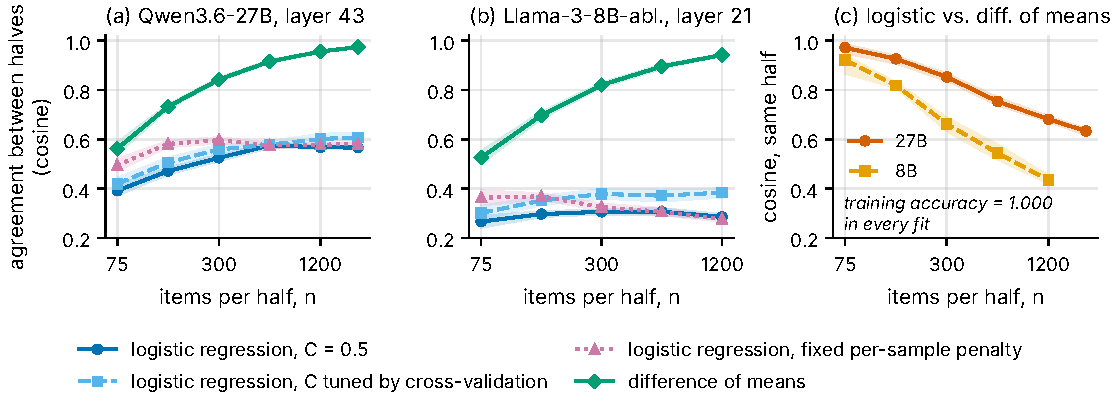
\includegraphics[width=\linewidth]{fig_estimator}
\caption{\textbf{Logistic directions do not reproduce; difference-of-means directions do.} (a, b) Agreement between directions fitted on two disjoint halves of the estimator pool (cosine, averaged over emotions and ten splits) against the number of items per half. Difference of means rises towards 1; logistic regression levels off near 0.6 on the 27B and near 0.3 on the 8B, whether its penalty is fixed, tuned or held constant per item. (c) Within one half, the logistic direction starts close to the difference-of-means direction and drifts away as $n$ grows, while every logistic fit classifies its training half perfectly. Bands are bootstrap 95\% intervals over splits.}
\label{fig:estimator}
\end{figure}

\paragraph{The test: do two independent halves agree?} We split the estimator pool into two halves with no item in common, fit the same estimator on each, and take the cosine between the two directions, averaged over the six emotions and ten random splits. If an estimator measures something stable in the model, this agreement should rise towards 1 as the halves grow. Difference of means does: at the 27B focus layer (layer 43) with $n = 2000$ items per half it reaches 0.974, against 0.566 for logistic regression with the usual penalty ($C = 0.5$; Figure~\ref{fig:estimator}a). At layer 54 the two numbers are 0.979 and 0.554, and on the 8B at $n = 1200$ they are 0.941 and 0.286 (Figure~\ref{fig:estimator}b).

\paragraph{Changing the penalty does not fix it.} Logistic regression includes a penalty that keeps its coefficients small; $C$ sets how weak it is. Choosing $C$ for every fit by cross-validation, as ridge-tuned probes do \citep{gao2026raptor}, reaches only 0.61 (27B) and 0.38 (8B). Holding the penalty per item constant as $n$ grows ($C_n = 0.5\,N_{\mathrm{ref}}/n$, $N_{\mathrm{ref}} = 600$ or 2000) leaves the curve flat on the 27B (0.581 at both $n = 150$ and 2000) and falling on the 8B (to 0.276 at $n = 1200$).

\paragraph{Why: the classifier separates its training data perfectly.} When there are fewer items than dimensions ($n \le 2000$ against $d = 5120$ on the 27B), a hyperplane can usually be found that puts every training item on its correct side. Every logistic fit we ran did this: training accuracy was exactly 1.000 in every fit, at every $n$, on both models and for every penalty we tried. Once the data are separated, many directions classify them perfectly, and the penalty, not the data, picks one of them: the penalty's \emph{tie-break}. Two checks support this reading. Weakening the penalty a hundred- or a thousandfold barely moves the direction (cosine 0.96 to the $C = 0.5$ fit on the same half) and does not make it more reproducible (0.52 against 0.58 at $n = 2000$). And within one half the logistic direction starts close to the difference-of-means direction and drifts away from it as $n$ grows, from 0.97 to 0.63 on the 27B and from 0.92 to 0.43 on the 8B (Figure~\ref{fig:estimator}c). The plain, unstandardised mean difference used by contrastive activation addition \citep{rimsky2023caa} agrees with the logistic direction at only 0.43 (27B) and 0.33--0.37 (8B) at $n = 2000$. We do not claim that the fits reach the maximum-margin limit, since the weak-penalty fits stop at the solver's tolerance.

\paragraph{How general is this?} Separation comes from the regime, not from logistic regression itself. For points in general position, any two-class labelling of at most $d + 1$ points can be separated by a hyperplane \citep{cover1965geometrical,candes2020phase}. Activations need not be in general position, which is why we checked separation directly instead of assuming it. When we project the 27B activations onto their top 100 principal components, so that $n$ is up to 20 times the dimension, the fits stop separating their halves from $n = 600$ (training accuracy 0.974 at $n = 2000$). The logistic direction then becomes reproducible (0.90 against 0.94 for difference of means at $n = 2000$), and its cosine to the difference-of-means direction stays at 0.91--0.94 instead of falling.\footnote{These cosines are in standardised coordinates. Figure~\ref{fig:estimator} uses raw activation coordinates, in which the difference-of-means direction is $(\mu_+ - \mu_-)/\sigma^2$; the two conventions give different numbers but the same pattern.} The 8B behaves the same way (0.81 against 0.85). The instability therefore needs the $n < d$ regime, and our claim is limited to it; that regime is the common one, since probe pools are usually small compared with model width.

\paragraph{Does it matter for reading?} As a classifier, logistic regression is the better estimator: on held-out items at the 27B focus layer its six-way accuracy is 0.82--0.94, against 0.79--0.88 for difference of means ($n = 75$ to 2000), and the two estimators' scores for the same held-out items correlate at 0.90--0.96. The coefficient row is a good classifier and a poor direction, the distinction \citet{marks2023geometry} drew; the instability matters when the direction itself is reused to steer or erase, as in the rest of this paper. From here on, every direction is a difference of means.

% ---------------------------------------------------------------------------------------
\section{B's response to A's steering}
\label{sec:transfer}
\begin{figure}[t]
\centering
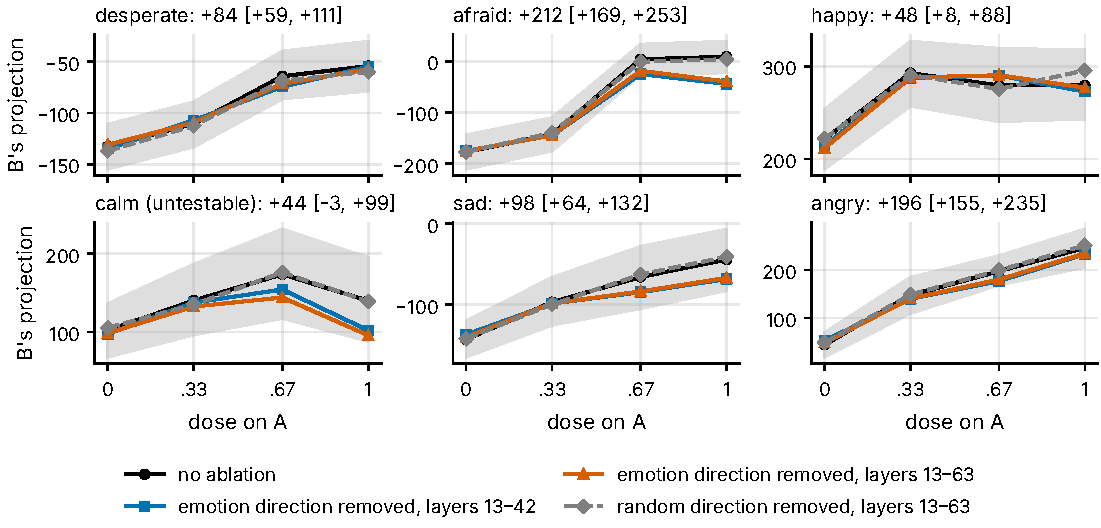
\includegraphics[width=\linewidth]{fig_dose}
\caption{\textbf{B's present-emotion projection rises with A's dose for five emotions, and erasing the emotion direction flattens it only for afraid and sad.} Mean projection per dose (29 scenarios $\times$ 3 replicates) with no ablation (black, with its scenario-bootstrap 95\% band) and under the three ablation arms of B1c (Section~\ref{sec:ablations}). Titles give the slope with no ablation and its 95\% interval. Happy levels off after the first step and calm turns down at the top dose. Whether two arms differ is decided by paired tests (Section~\ref{sec:ablations}), not by comparing the curves.}
\label{fig:dose}
\end{figure}

We first ask whether B's present-emotion projection moves at all. For each emotion we fit the dose-response slope with no ablation, which we call the \emph{none} arm. Under the pre-registered rule, an emotion is \emph{testable}, and enters the ablation tests of Section~\ref{sec:ablations}, only if this slope's interval excludes zero. The projection rises with A's dose for desperate, afraid, happy, sad and angry, with slopes from $+48$ to $+212$ probe units per unit dose; calm's slope ($+44$ $[-3, +99]$) does not exclude zero, so calm is untestable (Figure~\ref{fig:dose}). A single slope summarises two of the curves poorly: happy rises over the first dose step ($+71$ $[+50, +94]$) and not over the last ($+0$ $[-24, +25]$), and calm rises and then falls back. The steering does reach A's text. Our \emph{steering check} asks the model which of six emotions A is feeling; in each of the three main runs, the probability it gives to the steered emotion rises with the dose for all six emotions. A follow-up run with freshly sampled replies from B finds the same five testable emotions, and the same two blocked emotions in Section~\ref{sec:ablations}. On the 8B the same five emotions respond, but the steering there is half as strong and less specific, so we compare only the pattern.

\paragraph{What the probe measures.} B's other-speaker projection, which reads the interlocutor's emotion, rises with A's dose as well: slopes $+59$, $+119$, $+65$, $+93$ and $+96$ for desperate, afraid, happy, sad and angry, against $+84$, $+212$, $+48$, $+98$ and $+196$ for the present-emotion projection. The present-emotion projection therefore cannot tell B's own state apart from B's representation of A's state. A third reading is also open: B's reply is read with A's message in context, so the projection may partly reflect A's words themselves. We therefore report a receiver-side, affect-related response. We do not claim that affect is transferred to B or that B's own state changes. An earlier claim that the present-emotion shift exceeds the other-speaker shift did not survive a probe fitted on separate data (report 18 in the supplementary material).

% ---------------------------------------------------------------------------------------
\section{Three pre-registered ablations}
\label{sec:ablations}
If the emotion direction is what carries A's affect to B, removing it from what B reads should flatten B's response. To \emph{ablate} a direction we project it out of B's residual stream at the tokens of A's message (\emph{A's span}) while B reads that message and writes its reply, at every layer from 13 to 63; every one of these layers passes the pre-registered reproducibility gate (split-half cosine $\ge 0.80$). B's reply is then re-read with no hooks and scored as in Section~\ref{sec:transfer}. We report the \emph{blocked fraction}: how much an ablation lowers B's slope, as a fraction of the none-arm slope (0 means no change, 1 means the slope is gone, and a negative value means the slope grew). Significance is decided on the paired slope difference in probe units (Table~\ref{tab:slopes}); the fraction is a readable scale whose ranges understate uncertainty where the none-arm slope is imprecise (happy, calm).

\paragraph{Controls, and checking the instrument.} Controls remove something without emotional meaning. A \emph{random direction}, or a random set of $k$ orthogonal directions (a random $k$-frame), is the usual control. A \emph{permuted-label} control runs the same estimator on the same activations after shuffling the emotion labels, so it shares the pool's geometry but carries no emotion information. The \emph{top principal direction} is the direction along which A's span varies most, found without labels. To check that an ablation removes what it targets, we apply the forced-choice readout to A's span with the ablation switched on; the \emph{readable affect removed} is how much that readout drops at the top dose. An ablation that also shifts this readout at dose 0 changes the very thing used to check it, so its result cannot be read (the instrument fails). Each design's hypotheses, decision rule and checks were committed before it ran; Table~\ref{tab:map} separates these registered tests from later additions.

\begin{table}[t]
\centering\footnotesize
\caption{\textbf{Map of the evidence.} Every row ablates at A's span, layers 13--63, on the 27B unless marked. Numbers are blocked fractions of the none-arm slope; $\q$: BH-FDR $q < 0.05$ over the five testable emotions; $\ua$: unadjusted 95\% interval excludes zero. ``Addendum'': run after review under a written addendum to the pre-registration, committed before launch.}
\label{tab:map}
\setlength{\tabcolsep}{3.3pt}
\begin{tabularx}{\linewidth}{@{}>{\raggedright\arraybackslash}p{0.85cm}>{\raggedright\arraybackslash}p{1.38cm}>{\raggedright\arraybackslash}p{3.45cm}>{\raggedright\arraybackslash}p{2.2cm}Y@{}}
\toprule
Design & Status & Erased (compared with) & Verdict & What is blocked \\ \midrule
B1c & registered & emotion direction, rank 1 (random direction) & H1: rank 1 is not enough & afraid $0.21\q$, sad $0.33\q$ \\
B1d & registered & affect subspace, rank 5 (permuted-label subspace) & instrument failed & vs.\ none: sad $0.54\q$, angry $0.40\q$; the permuted subspace itself: afraid $0.23\q$, sad $0.27\q$, angry $0.23\q$ \\
B1d & addendum & random 23-frame; 4 new label shuffles (none) & descriptive & 23-frame: nothing; shuffles: angry 4/4, sad 3/4, afraid 1/4 ($\ua$) \\
B1e & registered & emotion direction, rank 1 (permuted-label direction) & H3: block survives & afraid $0.25\q$, sad $0.29\q$ \\
B1e & addendum & as B1e, 10 re-splits of the pool & descriptive & sad 10/10 (median 0.35); afraid 9/10 (0.18), steering check 4/10 \\
8B & not registered & B1c and B1e designs & B1c: instrument failed; B1e: H3 & sad $0.31\ua$ / $0.36\q$; afraid $0.15\ua$ / 0.14 \\
\bottomrule
\end{tabularx}
\end{table}

\paragraph{B1c: erasing the emotion direction.} Does the rank-1 emotion direction carry most of B's response? The registered rule compared it with a random direction by the median blocked fraction over testable emotions: H1 (rank 1 is not enough) if the median is at most 0.50, H1$'$ (rank 1 carries it) if at least 0.80. The median is 0.09 (95\% interval $[0.04, 0.25]$), so the verdict is H1: 91\% of the response remains. Per emotion the fractions are 0.06, 0.21, 0.05, 0.33 and 0.09 (desperate, afraid, happy, sad, angry); only afraid ($q = 0.001$) and sad ($q = 0.048$) pass the false-discovery threshold. Against the none arm the median is also 0.09, and afraid passes while sad does not ($q = 0.115$). The random direction removes twice the norm and changes nothing ($q \ge 0.26$), and stopping the ablation at layer 42 instead of 63 makes no detectable difference.

\paragraph{B1d: erasing the five-dimensional affect subspace.} The six emotions' average activations span a five-dimensional \emph{affect subspace} (16--21\% of the pool's variance). The registered test compared it with a permuted-label subspace of the same rank. The instrument failed: the affect subspace removes at least 80\% of the readable affect for only three of six emotions, and it shifts the readout already at dose 0 (desperate 0.11 to 0.50), so the registered decision is void and what follows is descriptive. Against the none arm (Figure~\ref{fig:blocked}), the affect subspace blocks sad (0.54) and angry (0.40) at $q < 0.001$. The permuted-label subspace, which contains no emotion information, blocks afraid (0.23), sad (0.27) and angry (0.23) at $q = 0.001$, 0.035 and 0.013, while shifting the dose-0 readout by at most 0.08. A random 5-frame, with half its footprint, blocks nothing ($q \ge 0.51$), and neither does a random 23-frame whose footprint matches the permuted subspace ($q \ge 0.71$). Which emotions it blocks depends partly on the shuffle: four fresh shuffles block angry in all four, sad in three, afraid in one, and all three together in only one (Table~\ref{tab:permnull}). The three-emotion pattern is one draw; the block on angry and sad recurs. The registered contrast, affect minus permuted subspace, passes no false-discovery threshold ($q = 0.051$).

\begin{figure}[t]
\centering
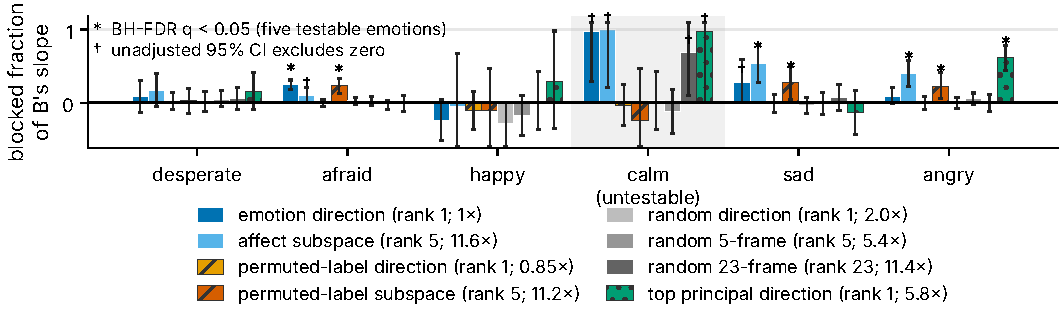
\includegraphics[width=\linewidth]{fig_blocked}
\caption{\textbf{Every arm against baseline: random controls never block, but a permuted-label subspace does.} Blocked fraction of B's slope for every ablation of the three 27B experiments; the legend gives each arm's rank and its footprint relative to the emotion direction. Error bars are the paired contrast's 95\% interval divided by the none-arm slope; bars and whiskers are clipped at the axis limits (calm, happy). Calm is untestable and shaded. Numbers are in Tables~\ref{tab:arms} and~\ref{tab:slopes}.}
\label{fig:blocked}
\end{figure}

\paragraph{B1e: a permuted-label control at rank 1.} Registered after B1d, this design asks about the two emotions B1c blocked. H3 states that the emotion direction blocks more than a permuted-label direction for both afraid and sad. The permuted-label direction is almost orthogonal to the emotion direction (cosine 0.004), removes 0.85$\times$ its norm, and changes nothing on its own (it removes at most 9\% of the readable affect). Against it the emotion direction blocks afraid by 0.25 $[0.17, 0.33]$ and sad by 0.29 $[0.07, 0.56]$ ($q = 0.001$ and 0.028), so the verdict is H3. We then re-split the probe pool ten times, re-estimating every direction and the readout probe (Table~\ref{tab:draws}). Sad's block has a median of 0.35 (range 0.24--0.56), is significant in all ten draws, and its steering check passes in all ten. Afraid's block has a median of 0.18 (0.07--0.23) and is significant in nine draws, but its steering check passes in only four, so afraid is less reliable. The top principal direction, with 5.8$\times$ the footprint, blocks angry (0.61, $q = 0.001$) but leaves afraid and sad untouched, although it removes 79\% and 71\% of their readable affect: removing readable affect and blocking B's response are different things. It also changes B's text (replies two words longer, perplexity 3.7 lower), whereas the blocking subspace arms keep B's replies within 1.2 words and 0.13 perplexity of baseline (Table~\ref{tab:coherence}).

\paragraph{Replication on the 8B.} Neither run was pre-registered. With B1c's design the 8B blocks the same two emotions by unadjusted intervals (afraid 0.15, sad 0.31), the other three being too wide to tell; its instrument check failed because the upper layers change the readout by nothing measurable and the strict rule has no tolerance band. With B1e's design it gives H3 (sad 0.36, $q = 0.002$; afraid 0.14, $q = 0.08$, no block against the none arm), but its control matches the footprint only on average. Only sad's block replicates across models on both designs.

% ---------------------------------------------------------------------------------------
\section{What the controls teach}
\label{sec:controls}
Figure~\ref{fig:blocked} puts every arm on one scale. The random direction, the random 5-frame, the footprint-matched random 23-frame and the permuted-label direction block nothing. The permuted-label subspace blocks three emotions at the false-discovery threshold, at about half the affect subspace's size on the two they share (0.51 and 0.57 of it), and the top principal direction blocks angry. A study with only random controls would have called the affect subspace's blocks emotion-specific. Removing more norm is not what makes a control bite: the random 23-frame removes as much as the permuted subspace and is inert. Across five shuffles the permuted subspace blocks angry, sad and afraid in that order of frequency (5, 4, 2), the same order as the affect subspace's own blocks, which suggests that an emotion's place in the pool's geometry matters more than the labels (exploratory). Rank, construction and footprint remain confounded: the inert permuted direction is rank 1 and variance-scaled, while the permuted subspace is rank 5 and spanned by raw class means. Intermediate ranks (2 or 3), a random frame inside the pool's top principal subspace, and many more shuffles would separate these factors; we have not run them.

\paragraph{Recommendations, by use.}
\begin{itemize}[leftmargin=1.2em,itemsep=1pt,topsep=2pt]
\item \emph{Classifying or decoding a state:} logistic regression is fine and often better (Section~\ref{sec:estimator}).
\item \emph{A scalar readout:} either estimator; their scores correlate at 0.90--0.96. If readouts are compared across separate fits, prefer difference of means.
\item \emph{Steering or erasing:} use difference of means, or logistic regression in a low-dimensional space where the data are not separable, and report disjoint-half reproducibility.
\item \emph{Controls for an ablation:} beside a random direction, run the same estimator on permuted labels at the rank of the intervention, over several shuffles; report every arm's footprint; and check the manipulation with an instrument that does not share the ablation's target.
\end{itemize}

% ---------------------------------------------------------------------------------------
\section{Limitations}
\label{sec:limits}
\emph{Construct.} The present-emotion projection does not separate B's own state from B's representation of A's state or from A's words in B's context (Section~\ref{sec:transfer}). \emph{Behaviour.} We did not test whether B's decisions or the content of its replies change; the coherence measures in Table~\ref{tab:coherence} are sanity checks, not behavioural outcomes. \emph{Text channel.} Three designs that replaced A's message with a rewrite failed their own manipulation check, so whether a paraphrase of A's message without affective cues removes B's response is untested. \emph{Generality.} One model plays both roles in single-turn exchanges over 29 scenarios, and one probe pool underlies all 27B ablations; the ten re-splits measure sensitivity to how that pool is split, not to new pools or scenario families. \emph{Second model.} The 8B is an abliterated model (its refusal direction removed), its steering is weaker and less specific, and its runs were not pre-registered. \emph{Controls.} The random frames and the permuted-label direction are one draw each and the permuted subspace has five; the addendum contrasts are unadjusted, and multiplicity is controlled within experiments, not across the three experiments and two models. Layers below 13 were not ablated.

\section{Conclusion}
The two failures we found are the same failure seen twice. A logistic direction on separable activations is set by the penalty's tie-break, so two independent fits agree only as far as their tie-breaks do; and a control is informative only if it is built the way the intervention was. A random vector is not built from the data, so it stays inert and misses what a control built from the same activations catches. Studies that read or erase concept directions should report disjoint-half reproducibility, estimate directions with an average rather than a separating hyperplane, and run permuted-label controls at the rank of the intervention. For affect, the rank-1 direction carries 24--56\% of sad's response across the ten 27B draws and only sad's block carries over to the 8B; afraid's block is less reliable, and whose state the probe reads remains open.

\bibliographystyle{plainnat}
\bibliography{references}

% =======================================================================================
\appendix
\section{Reproducibility statement}
\label{app:repro}
Before submission, the paper went through two rounds of internal adversarial review by language-model reviewers (three reviewers, a citation audit, a numerical audit and an area chair in each round; all in the supplementary material); it was then peer-reviewed at the workshop, and this version addresses those reviews. Every number is registered in the claim registry under the identifier listed in Appendix~\ref{app:registry}; the registry is machine-checked against the result files. Figures and tables are generated from those files by \texttt{paper\_figures\_cr.py}, \texttt{paper\_revision\_stats.py} and \texttt{paper\_appendix\_tables.py}.

Code, pre-registrations, result files and the claim registry are in the supplementary material (research-use licence). Models: Qwen3.6-27B revision \texttt{6a9e13bd} and Llama-3-8B-Instruct-abliterated revision \texttt{dd67dd05}, run with torch 2.11.0+cu130 and transformers 5.14.1 on one NVIDIA RTX PRO 6000 (96\,GB) per run; a 27B ablation experiment takes about two hours (432, 360 or 288 arm-rows of 29 scenarios each, 144 and 72 for the post-review runs, 19--21\,s per arm-row), the 8B one under an hour. Seeds: pool generation seed 0; per-generation seeds are a CRC32 of (seed, emotion, dose, replicate, arm, part) with the arm field empty for the receiver's reply so that arms share random numbers; ten split seeds (0--9) for every split-half number; bootstrap seed 0 with 5{,}000 draws. Three further sets of 27B runs were added after review (2026-09-06, pre-registered as addenda to PREREG\_B1d and PREREG\_B1e before launch): ten B1e draws that re-split the same probe pool with split seeds 1--10 (the original run used 0), restricted to afraid and sad and the arms none, emotion direction and permuted-label direction, so that the steering direction, the per-layer ablation directions, the control and the readout probe are all re-estimated per draw; one B1d run with the arms none and random frame only, the frame's rank raised from 5 to 23 so that its expected footprint matches the permuted-label frame's ($5 \times (6.7/3.15)^2 \approx 23$); and four B1d runs with the permuted-label frame only, each with a fresh label permutation (permutation seeds 1--4; the paper's frame used seed 0), contrasted against the B1d run's stored none arm. Generation seeds, doses, replicates and scenarios are unchanged, so each draw's none arm is a fresh sample of the same design. Hyperparameters: doses $\{0, 0.33, 0.67, 1\}$ at a fixed activation-RMS scale, three replicates, 29 scenarios, 110 new tokens per message in the ablation runs (240 in the estimator pool) at temperature 0.9; logistic regression with lbfgs, max\_iter 3000, $C \in \{0.5,\ C_n = 0.5\,N_{\mathrm{ref}}/n \text{ with } N_{\mathrm{ref}} \in \{600, 2000\},\ 50,\ 500\}$ and cross-validated $C$ on a decade grid scored for accuracy; split-half $n \in \{75, 150, 300, 600, 1200, 2000\}$ per half where the pool allows. Statistics: scenario-blocked percentile bootstraps because scenarios are the sampling unit; between-arm contrasts paired within scenario and dose; two-sided bootstrap $p$-values with Benjamini--Hochberg over the testable emotions of one arm; every interval in the paper is such a bootstrap and every count of runs is stated. The pre-registered decision medians recompute numerator and denominator in every bootstrap draw; per-emotion blocked-fraction ranges divide the contrast's interval by the point estimate of the none-arm slope. The probe pools and scenario lists are committed with the results.

\section{Details and defects recorded under review}
\label{app:details}
Each item below is in the registry note of the claim it qualifies.
\begin{itemize}[leftmargin=1.2em,itemsep=1pt,topsep=2pt]
\item \emph{B1c.} The contrast between the 30-layer and 51-layer windows was declared in the driver, not in the pre-registration; its null is unpowered for desperate and calm. The testability rule (none-arm CI excludes zero) is pre-registered (PREREG\_B1c \S5). Calm's contrast is the largest and is excluded by that rule; medians are reported with and without it (with calm: 0.15 against the random direction, 0.17 against baseline). Afraid's top-dose readout is non-monotone. The pre-registration stamp is empty because the driver resolved its path relative to the wrong directory; the document was on the machine one second before the run started, and its recorded version (\texttt{cc2dc32}, 19:22Z) precedes the run's start (19:32Z) in the supplementary-material history. The pool has 1,615 items against the registered 2,160; the false-discovery rate ran over five emotions rather than six. Re-running the decision contrast's BH adjustment over the pre-registered six-emotion family changes no verdict: afraid $q=0.001$, sad 0.030, calm 0.011, angry 0.093 (five-emotion family on the same recomputation: 0.001, 0.037, --, 0.103, against the driver's own bootstrap in Section~\ref{sec:ablations}, 0.001 and 0.048; \texttt{results/rev3/b1c\_fdr\_six\_family.json}).
\item \emph{B1d.} The permuted-label subspace removed only 6.5\% of afraid's readable affect and still blocked its response, so overlap with the readable-affect direction does not explain its blocking; recomputing the instrument share with each arm's own floor keeps three failures but changes which emotions fail. The median's confidence interval resamples scenarios only. The footprint-matched 23-frame was run after review with only the none and random arms; it shifts calm, the untestable emotion, by $-30$ $[-55, -4]$ slope units (calm's own slope is $+44$ $[-3, +99]$), reported in Table~\ref{tab:arms} in parentheses and outside the false-discovery family. The four fresh label permutations (Table~\ref{tab:permnull}) ran the permuted arm only, 72 arm-rows each; their dose-0 readout shifts are at most 0.30 (desperate, permutation 2; the paper's frame at most 0.08), their contrasts are unadjusted (one arm, five testable emotions, no family declared in the addendum), and calm, untestable, moves by 58--142\% of its own imprecise slope, outside the family.
\item \emph{B1e.} The control removes less norm than the emotion direction and less than B1c's inert random direction (1.22), so it is a fitted label-free null, not a footprint-matched one. The rule tests the point fraction and sad's range starts at 0.07. The secondary readout on B's reply contradicts afraid's block and agrees for sad. The control's cosine to the emotion direction (0.004) was measured by the pre-launch verifier and is not stamped in the result file.
\item \emph{Direction draws.} The ten re-splits reuse the pool file under a per-draw tag; draw 4 ran on a different machine from draws 1--3 after a rebalancing, with the same seeds. Afraid's manipulation check is a CI rule on the A-span readout slope; in the six failing draws that slope is $-0.02$ to $+0.09$ with intervals that include zero, two of them by less than 0.01, so the verdict split (four H3, six instrument\_failed) is a property of the gate, not of the decision contrast, which is significantly negative in nine draws. The addendum attaches no verdict to the ensemble; the medians and ranges are descriptive. The permuted direction against baseline reaches significance in two of the twenty emotion-draws (afraid, draw 6, $+6.5\%$ of the slope removed; sad, draw 3, $-13\%$, an amplification).
\item \emph{8B replications.} Both are out-of-pre-registration replications (the documents name the 27B and its layers). The steering manipulation is half as strong and less specific on the 8B, afraid's readout sits below chance, and slopes are unnormalised probe scores, so only patterns are compared. In B1e on the 8B the control is matched on average only (sad 0.86$\times$), both directions remove about the isotropic norm, and B1c's random direction already reproduced the contrasts; afraid does not block against baseline there.
\item \emph{Estimator study.} The weak-penalty arms ($C = 50$ and $500$) give the same solution to three decimals, so they are tolerance-limited and bound nothing about the $C \to \infty$ limit. The fixed per-sample penalty has a significant dip of $-0.021$ at $n = 600$ on the 27B focus layer, falls once and then stays flat at layer 54, and rises at layer 16. Cross-estimator cosines use subsamples that overlap by about half the pool, so their intervals overstate precision. The layer-43 and layer-54 files come from three driver builds; the shared cells agree bit for bit.
\end{itemize}

\section{Additional tables}
\label{app:tables}

\begin{table}[H]\centering\footnotesize
\caption{Pre-registered decision contrasts, as blocked fractions of the none-arm slope (B1c: emotion direction $-$ random direction; B1d: affect subspace $-$ permuted-label subspace; B1e: emotion direction $-$ permuted-label direction). $\q$: BH-FDR $q<0.05$ within the contrast's own family of five testable emotions; $\ua$: unadjusted CI excludes zero only. Calm ($u$) is untestable.}
\label{tab:decision}
\begin{tabular}{lcccccc}\toprule
 & desperate & afraid & happy & calm$^{u}$ & sad & angry \\ \midrule
B1c: emotion dir $-$ random dir & 0.06 & 0.21$\q$ & 0.05 & (0.94)$\ua$ & 0.33$\q$ & 0.09 \\
B1d: affect subspace $-$ permuted subspace & 0.14 & $-$0.13$\ua$ & 0.05 & (1.56)$\ua$ & 0.26$\ua$ & 0.17$\ua$ \\
B1e: emotion dir $-$ permuted-label dir & 0.06 & 0.25$\q$ & $-$0.14 & (1.02)$\ua$ & 0.29$\q$ & 0.09 \\ \bottomrule
\end{tabular}
\end{table}

\begin{table}[H]\centering\footnotesize
\caption{Every ablation arm against baseline (none), as blocked fractions of the none-arm slope, scenario-blocked and dose-paired; marks as in Table~\ref{tab:decision}, families being the arm's five testable emotions. ``hs'': hidden states (layers) ablated.}
\label{tab:arms}
\resizebox{\textwidth}{!}{\begin{tabular}{llcccccc}\toprule
run & arm $-$ none & desperate & afraid & happy & calm$^{u}$ & sad & angry \\ \midrule
Exp.~1 & emotion direction (rank 1, layers 13--63) & +0.08 & +0.24$^{*}$ & -0.24 & (+0.98)$^{\dagger}$ & +0.28$^{\dagger}$ & +0.09 \\
Exp.~1 & emotion direction (rank 1, layers 13--42) & +0.03 & +0.27$^{*}$ & -0.11 & (+0.79)$^{\dagger}$ & +0.33$^{*}$ & +0.12$^{*}$ \\
Exp.~1 & random direction (rank 1) & +0.02 & +0.03 & -0.28 & (+0.04) & -0.04 & -0.00 \\
Exp.~2 & affect subspace (rank 5) & +0.16 & +0.11$^{\dagger}$ & -0.05 & (+1.32)$^{\dagger}$ & +0.54$^{*}$ & +0.40$^{*}$ \\
Exp.~2 & permuted-label subspace (rank 5) & +0.03 & +0.23$^{*}$ & -0.10 & (-0.24) & +0.27$^{*}$ & +0.23$^{*}$ \\
Exp.~2 & random 5-frame (rank 5) & +0.05 & +0.02 & -0.17 & (-0.12) & -0.01 & +0.06 \\
Exp.~2 & random 23-frame, footprint-matched (rank 23) & +0.06 & -0.03 & +0.03 & (+0.68)$^{\dagger}$ & +0.07 & +0.00 \\
Exp.~3 & permuted-label direction (rank 1) & +0.02 & -0.00 & -0.10 & (-0.04) & -0.01 & +0.00 \\
Exp.~3 & top principal direction (rank 1) & +0.16 & -0.01 & +0.30 & (+0.98)$^{\dagger}$ & -0.13 & +0.61$^{*}$ \\
\bottomrule\end{tabular}}
\end{table}

\begin{table}[H]\centering\footnotesize
\caption{The directions and subspaces: rank; footprint (norm removed per masked position, averaged over ablated layers) with its ratio to the emotion direction in the same run; largest dose-0 shift of the A-span readout; share of readable affect removed at the top dose (range over emotions). $^{\ddagger}$: the 23-frame's run has no emotion arm; its ratio uses the B1d run's emotion direction, and the two runs' none arms agree bit for bit.}
\label{tab:dirs}
\resizebox{\textwidth}{!}{%
\begin{tabular}{llcccc}\toprule
run & arm & rank & footprint (ratio) & dose-0 shift & readable affect removed \\ \midrule
B1c & emotion direction & 1 & 0.46--0.66 (1) & $\le 0.08$ & 0.16--0.79 \\
B1c & random direction & 1 & 1.15--1.26 (2.0) & $\le 0.01$ & $\le 0.03$ \\
B1d & affect subspace & 5 & 6.9 (11.6) & $+0.39$ / $-0.25$ & 0.11--1.25 \\
B1d & permuted-label subspace & 5 & 6.5--6.9 (11.2) & $\le 0.08$ & 0.07--0.52 \\
B1d & random 5-frame & 5 & 3.1--3.2 (5.4) & $\le 0.01$ & $\le 0.03$ \\
B1d & random 23-frame, footprint-matched & 23 & 6.7--6.9 (11.4)$^{\ddagger}$ & $\le 0.01$ & $\le 0.13$ \\
B1e & permuted-label direction & 1 & 0.50 (0.85; afraid 0.84, sad 0.77) & $\le 0.01$ & $\le 0.09$ \\
B1e & top principal direction & 1 & 3.47 (5.8) & $+0.55$ / $-0.28$ & 0.01--1.5 \\ \bottomrule
\end{tabular}}
\end{table}

\begin{table}[H]\centering\footnotesize
\caption{Direction-resampling draws (PREREG\_B1e addendum 3): blocked fractions of the none-arm slope for afraid and sad in ten re-splits of the probe pool (split seeds 1--10; ``Draw 0'' is the run in Table~\ref{tab:decision}), with the median and range across draws, the number of draws whose contrast's unadjusted scenario-bootstrap CI lies below zero (the draws ran two emotions, so no five-emotion family exists; no adjustment is applied), and the number of draws in which the emotion's steering check (the A-span readout responds to A's own steering) passes.}
\label{tab:draws}
\begin{tabular}{llrrrrr}
\toprule
Emotion & Contrast & Draw 0 & Median & Range & Sig.\ neg. & Gate passes \\
\midrule
afraid & emotion $-$ permuted-label & 0.25 & 0.18 & [0.07, 0.23] & 9/10 & 4/10 \\
 & emotion $-$ none & 0.24 & 0.19 & [0.08, 0.23] & 10/10 &  \\
 & permuted-label $-$ none & 0.00 & 0.02 & [-0.04, 0.07] & 1/10 &  \\
sad & emotion $-$ permuted-label & 0.29 & 0.35 & [0.24, 0.56] & 10/10 & 10/10 \\
 & emotion $-$ none & 0.28 & 0.35 & [0.23, 0.44] & 10/10 &  \\
 & permuted-label $-$ none & -0.01 & -0.01 & [-0.13, 0.09] & 0/10 &  \\
\bottomrule
\end{tabular}

\end{table}

\begin{sidewaystable}\centering\footnotesize
\caption{Every ablation arm against baseline in slope units (arm $-$ none, scenario-blocked and dose-paired, with 95\% bootstrap CIs), the numbers behind Table~\ref{tab:arms} and Figure~\ref{fig:blocked}; significance is decided on these differences. The first row is the none-arm slope each blocked fraction divides by. Calm ($u$) is untestable.}
\label{tab:slopes}
\resizebox{\textheight}{!}{\begin{tabular}{llcccccc}
\toprule
run & arm $-$ none (slope units) & desperate & afraid & happy & calm$^{u}$ & sad & angry \\
\midrule
none-arm slope & & +84 [+59, +111] & +212 [+169, +253] & +48 [+8, +88] & +44 [-3, +99] & +98 [+64, +132] & +196 [+155, +235] \\
\midrule
Exp.~1 & emotion direction (rank 1, layers 13--63) & -7 [-26, +11] & -52 [-66, -37] & +11 [-2, +25] & -43 [-74, -13] & -28 [-58, -0] & -18 [-40, +2] \\
Exp.~1 & emotion direction (rank 1, layers 13--42) & -3 [-23, +18] & -58 [-71, -44] & +5 [-10, +20] & -35 [-61, -9] & -32 [-57, -8] & -23 [-44, -4] \\
Exp.~1 & random direction (rank 1) & -2 [-13, +9] & -7 [-16, +3] & +14 [-0, +28] & -2 [-19, +16] & +4 [-7, +15] & +1 [-14, +15] \\
Exp.~2 & affect subspace (rank 5) & -14 [-34, +4] & -23 [-45, -0] & +3 [-33, +36] & -58 [-95, -24] & -52 [-77, -27] & -78 [-113, -44] \\
Exp.~2 & permuted-label subspace (rank 5) & -2 [-17, +12] & -50 [-70, -27] & +5 [-23, +33] & +11 [-21, +40] & -27 [-49, -5] & -44 [-80, -12] \\
Exp.~2 & random 5-frame (rank 5) & -4 [-14, +5] & -4 [-17, +9] & +8 [-5, +21] & +5 [-8, +19] & +1 [-13, +16] & -12 [-26, +4] \\
Exp.~2 & random 23-frame, footprint-matched (rank 23) & -5 [-18, +8] & +6 [-7, +19] & -1 [-21, +18] & -30 [-55, -4] & -7 [-24, +11] & +0 [-22, +22] \\
Exp.~3 & permuted-label direction (rank 1) & -2 [-12, +8] & +1 [-10, +11] & +5 [-7, +17] & +2 [-11, +14] & +1 [-11, +13] & -1 [-18, +17] \\
Exp.~3 & top principal direction (rank 1) & -14 [-35, +7] & +2 [-21, +25] & -14 [-47, +17] & -43 [-91, -0] & +13 [-17, +43] & -120 [-154, -87] \\
\bottomrule
\end{tabular}
}
\end{sidewaystable}

\begin{table}[H]\centering\footnotesize
\caption{Coherence of B's replies per arm, averaged over all 72 (emotion, dose, replicate) arm-rows: mean words, degenerate and refusal rates, distinct-2 and the recorded perplexity of the reply. $\ua$: the paired arm-minus-none difference over the 72 cells has a bootstrap CI excluding zero. The blocking subspace arms differ from baseline by at most 1.2 words and 0.13 in perplexity; the top principal direction lowers perplexity to 11.2 and lengthens replies, so it changes B's output beyond the readout. All 27B runs share the none arm bit for bit.}
\label{tab:coherence}
\begin{tabular}{llrrrrr}
\toprule
run & arm & words & degenerate & refusal & distinct-2 & perplexity \\
\midrule
B1c & none (baseline) & 46 & 0.3\% & 0.3\% & 1.00 & 14.92 \\
B1c & emotion direction (hs 13--63) & 46 & 0.5\% & 0.5\% & 1.00 & 15.19 \\
B1c & emotion direction (hs 13--42) & 46 & 0.5\% & 0.5\% & 1.00 & 15.42$^{\dagger}$ \\
B1c & random direction & 46 & 0.3\% & 0.3\% & 1.00 & 14.72 \\
\midrule
B1d & none (baseline) & 46 & 0.3\% & 0.3\% & 1.00 & 14.92 \\
B1d & affect subspace (rank 5) & 45$^{\dagger}$ & 0.5\% & 0.5\% & 1.00 & 15.02 \\
B1d & permuted-label subspace (rank 5) & 45$^{\dagger}$ & 0.3\% & 0.3\% & 1.00$^{\dagger}$ & 15.05 \\
B1d & random 5-frame & 46$^{\dagger}$ & 0.4\% & 0.4\% & 1.00 & 14.46$^{\dagger}$ \\
\midrule
B1e & none (baseline) & 46 & 0.3\% & 0.3\% & 1.00 & 14.92 \\
B1e & permuted-label direction (rank 1) & 46 & 0.4\% & 0.4\% & 1.00 & 14.87 \\
B1e & top principal direction & 48$^{\dagger}$ & 0.0\%$^{\dagger}$ & 0.0\%$^{\dagger}$ & 1.00$^{\dagger}$ & 11.23$^{\dagger}$ \\
\midrule
B1d-23 & none (baseline) & 46 & 0.3\% & 0.3\% & 1.00 & 14.92 \\
B1d-23 & random 23-frame, footprint-matched & 46 & 0.3\% & 0.3\% & 1.00 & 14.80 \\
\bottomrule
\end{tabular}

\end{table}

\begin{table}[H]\centering\footnotesize
\caption{Permutation null for the permuted-label rank-5 subspace (PREREG\_B1d addendum 3): blocked fractions of the none-arm slope for the subspace in the main text (permutation seed 0) and for fresh label permutations run after review, each against the same stored none arm (identical generation seeds); $\ua$: scenario-blocked, dose-paired CI below zero, unadjusted. Calm ($u$) is untestable. Afraid, sad and angry are blocked together in only one of the four fresh permutations, so under the addendum's fixed reading the main-text subspace was an unlucky draw for that three-emotion pattern, which is downgraded to a single-realisation observation; per emotion, angry's block recurs in all five permutations, sad's in four and afraid's in two.}
\label{tab:permnull}
\begin{tabular}{lcccccc}
\toprule
permutation & desperate & afraid & happy & calm$^{u}$ & sad & angry \\
\midrule
0 (paper) & +0.03 & +0.23$^{\dagger}$ & -0.10 & (-0.24) & +0.27$^{\dagger}$ & +0.23$^{\dagger}$ \\
1 & -0.01 & +0.00 & +0.23 & (+1.25)$^{\dagger}$ & +0.40$^{\dagger}$ & +0.16$^{\dagger}$ \\
2 & -0.01 & +0.01 & -0.05 & (+0.95)$^{\dagger}$ & +0.12 & +0.20$^{\dagger}$ \\
3 & +0.05 & +0.02 & +0.13 & (+0.58) & +0.34$^{\dagger}$ & +0.19$^{\dagger}$ \\
4 & +0.17 & +0.14$^{\dagger}$ & -0.37 & (+1.42)$^{\dagger}$ & +0.35$^{\dagger}$ & +0.20$^{\dagger}$ \\
\midrule
median & +0.03 & +0.02 & -0.05 & +0.95 & +0.34 & +0.20 \\
blocks (CI $<0$) & 0/5 & 2/5 & 0/5 & 3/5 & 4/5 & 5/5 \\
\bottomrule
\end{tabular}

\end{table}

\section{Claim registry map}
\label{app:registry}
Identifiers in the claim registry (\texttt{docs/review/claims.json}) for the numbers in the main text; each points to the committed script, configuration and result file that produced the number. A trailing \texttt{*} denotes every identifier with that prefix.

{\footnotesize
\begin{tabularx}{\linewidth}{@{}p{0.43\linewidth}Y@{}}
\toprule
Claim (section) & Identifier(s) \\ \midrule
Disjoint-half cosine, 27B layer 43 (\S\ref{sec:estimator}) & \texttt{a2.focus\_dom\_split\_half}, \texttt{a2.focus\_logreg\_split\_half} \\
Disjoint-half cosine, 27B layer 54; 8B layer 21 & \texttt{a2f54.*}; \texttt{a2\_8b.*} \\
Cross-validated $C$ (27B; 8B) & \texttt{a2f.focus\_tuned\_c\_does\_not\_close\_gap}; \texttt{a2f8.lam\_declines} \\
Fixed per-sample penalty & \texttt{a2f.focus\_logreg\_fixed\_lambda\_flat}, \texttt{a2f2.lam\_anchor2000\_no\_rise}, \texttt{a2f54.lam\_declines\_anchor600}, \texttt{a2f8.lam\_declines} \\
Perfect separation in every fit & \texttt{a2m.separable\_every\_n}, \texttt{a2m.8b\_same\_regime}, \texttt{a2m.v2\_ten\_seeds} \\
Weak penalty, same direction & \texttt{a2m.weak\_penalty\_same\_direction} \\
Drift from difference of means (27B; 8B) & \texttt{a2m.logistic\_departs\_from\_dom}; \texttt{a2m.8b\_same\_regime} \\
Plain mean difference vs.\ logistic & \texttt{a2f.caa\_raw\_vs\_logreg\_raw}, \texttt{a2f8.cross\_estimator} \\
100-dimensional refit (27B; 8B) & \texttt{a2l.lowd\_recovers}; \texttt{a2l.8b\_lowd} \\
Held-out accuracy and score correlation & \texttt{a2l.heldout\_and\_projcorr} \\
Testable emotions; dose shape (\S\ref{sec:transfer}) & \texttt{b1c.verdict\_H1}; \texttt{rev.dose\_shape} \\
Follow-up run; determinism across runs & \texttt{b1f.*}; \texttt{b1d.replicates\_b1c\_arms} \\
8B response; other-speaker projection & \texttt{b1c8.transfer\_replicates}; \texttt{rev.other\_probe\_rises} \\
B1c verdict, median, per-emotion $q$ (\S\ref{sec:ablations}) & \texttt{b1c.verdict\_H1}, \texttt{b1c.median\_fraction}, \texttt{rev.b1c\_emo\_vs\_none\_fdr}, \texttt{b1c.partial\_block\_replicates} \\
B1c random control; layers 43--63; readout link & \texttt{rev.b1c\_random\_vs\_none}, \texttt{b1c.random\_control\_inert}; \texttt{b1c.no\_gain\_beyond\_layer42}; \texttt{b1c.readout\_residual} \\
B1d subspace geometry, instrument failure & \texttt{b1d.frame\_geometry}, \texttt{b1d.readout\_baseline\_shift}, \texttt{b1d.footprint} \\
B1d permuted subspace and random frames & \texttt{b1d.perm\_control\_blocks}, \texttt{rev.b1d\_controls\_vs\_none}, \texttt{b1d23.inert}, \texttt{b1d23.footprint\_matched} \\
B1d permutation null; registered contrast & \texttt{b1dperm.reading}, \texttt{b1dperm.counts}; \texttt{b1d.median\_fraction\_descriptive} \\
B1e verdict and permuted direction & \texttt{b1e.verdict\_H3}, \texttt{b1e.permdir\_inert} \\
B1e ten re-splits & \texttt{b1e10.sad\_stable}, \texttt{b1e10.afraid\_gate\_fragile} \\
Top principal direction & \texttt{b1e.pc1\_dissociation} \\
8B replications & \texttt{b1c8.verdict\_and\_block}, \texttt{b1e8.verdict\_H3\_matched} \\
Rewrite (text-channel) designs & \texttt{b1c.text\_arms\_uninterpretable} \\
\bottomrule
\end{tabularx}}

\end{document}
